
% Prof. Dr. Ausberto S. Castro Vera
% UENF - CCT - LCMAT - Curso de Ci\^{e}ncia da Computa\c{c}\~{a}o
% Campos, RJ,  2019 
% Disciplina: An\'{a}lise e Projeto de Sistemas
% Aluno:

\chapterimage{planejamento.png} % Table of contents heading image
\chapter{Etapa de Planejamento}


Neste capítulo serão  apresentados os motivos pelo qual se deve construir o sistema, além de mostrar também o orçamento , o desenvolvimento do plano de trabalho e por fim os benefícios que o sistema irá proporcionar.


\section{Solicita\c{c}\~{a}o do Sistema}
%%%%%%%%%%%%%%%%%%%%%%%%%%%%%%%
\begin{itemize}
\item \textbf{Responsável}
\subitem Luís Fernando Peixoto Cabral
	
\item \textbf{Necessidade de Negócio}
\subitem - O sistema tem como objetivo facilitar a comunicação entre os setores do hospital, permitindo assim aos funcionários uma melhor produtividade no trabalho, e consequentemente aos   pacientes um melhor atendimento.
Visa também facilitar no agendamento de consultas e exames, com opção prontamente para mudar de data e desmarca. Além de simplificar os pagamentos referente ao paciente 
\item \textbf{Requisitos do Negócio}
\subitem - Fornecer aos paciente a marcação de consultas e exames, através do site e por meio de aplicativo do próprio hospital.

\subitem - Oferecer suporte online, para sanar qualquer tipo de dúvida que o paciente possa ter.

\subitem - O sistema será capaz de permitir ao paciente, visualizar resultados de exames através do site e por aplicativo.

\subitem - Capaz de produzir relatórios de gestão para o setor administrativo.

\subitem - Permitir ao setor de farmácia o controle de estoque, além de proporcionar ao médico receitar remédios ao paciente pelo sistema.

\subitem - Fácil comunicação entre o setor de atendimento e o setor de pronto-socorro.

 \subitem - Proporcionar o socorro mais rápido  através da função de traçar rotas automaticamente pelo sistema, para o setor de pronto-socorro.

       
\item \textbf{Valor Agregado	}
\subitem - Diminuição de custo com papel, uma vez que o paciente pode ver resultado do exame on-line.

\subitem - Aumento no agendamento de consultas
       
\subitem - Diminuição de custo com estoque, através do controle de estoque.
       
 \subitem - Melhor gerenciamento de recurso proporcionado pelo sistema administrativo.

              
\item \textbf{Questões Especiais e Restrições}
\subitem - O sistema deverá ter um bom esquema de segurança uma vez que trabalha com dados de pacientes. 
\subitem - É de extrema importância que todos os funcionários tenha total compreensão das tecnologias e aplicações do sistema de seu determinado setor.
\subitem - É necessário que o  projeto deva ter um prazo mínimo de conclusão de um ano devido a complexidade do sistema, com vários subsistema e diversas funções incluídas.

\end{itemize}

\section{Custos: Desenvolvimento e Operacional}
%%%%%%%%%%%%%%%%%%%%%%%%%%%%%%%
\begin{itemize}

\item  \textbf{Desenvolvimento}

\subitem - Treinamento da equipe de  desenvolvimento
\subitem - Compras de hardwares e softwares
\subitem - Salário da equipe de desenvolvimento
\subitem - Equipamentos para escritório
\subitem - Treinamento de funcionários




\item  \textbf{Operacionais}

\subitem - Serviço de manutenção
\subitem - Atualizações de Software
\subitem - Licenciamento de Software 
\subitem - Salários da equipe operacional
\subitem - Gastos com comunicações 
\subitem - Treinamento de novos Usuários
\subitem - Gastos com energia elétrica
\end{itemize}

\section{Benef\'{\i}cios}
Nesta seção serão identificados os benefícios tangíveis e intangíveis que o sistema irá apresentar e listá-los a seguir.
       \subsection{Benef\'{\i}cios Tang\'{\i}veis}
       
       \begin{itemize}
       \item  Aumento de consultas e exames
       \item  Diminuição do tempo de espera em filas de atendimento
       \item  Socorro mais rápido
       \item  Sistema mais rápido
       \item   Divulgação dos resultados de exames mais rápido para o paciente
       \end{itemize}

       \subsection{Benef\'{\i}cios Intang\'{\i}veis}
       \begin{itemize}
       \item  Maior facilidade no agendamento de consulta e exames
       \item  Maior reconhecimento do hospital
       \item  Melhor gerenciamento de recursos
       \item  Pacientes mais satisfeitos
       \item  Maior facilidade para os funcionários realizar o trabalho 
       \item  Melhor comunicação entre os setores do hospital
       
       \end{itemize}


\section{Estudo de Viabilidade}
%%%%%%%%%%%%%%%%%%%%%%%%%%%%%%%

Serão apresentado a seguir o cronograma das atividades que serão realizadas para a construção do sistema, e a realização do cálculo de custo total do projeto. Através desta informações será possível determinar a viabilidade do projeto.
       \subsection{Calend\'{a}rio }
       \begin{table}[H]
              \centering
              \caption{Calendario com as fases de construção do sistema}

              \begin{tabular}{|c|c|}

              \hline
              {\ul \textbf{FASE}}                      & {\ul \textbf{DATA}}                        \\ \hline
              \textbf{Início do projeto} & \textbf{20 de fervereiro de 2020}    \\ \hline
              Planejamento               & 20/02/2020 á 22/07/2020     \\ \hline
              Analise                    & 22/07/2020 á 29/11/2020     \\ \hline
              Projeto                    & 29/11/2020 á 30/12/2020     \\ \hline
              Implementação              & 30/11/2021 á 21/05/2021     \\ \hline
              \textbf{Conclusão}         & \textbf{21 de maio de 2021} \\ \hline
              \end{tabular}
              \end{table}
       \subsection{Cronograma }
       \begin{figure}[H]
              \begin{center}
                  \caption{Cronograma do Projeto } \label{afp}
                  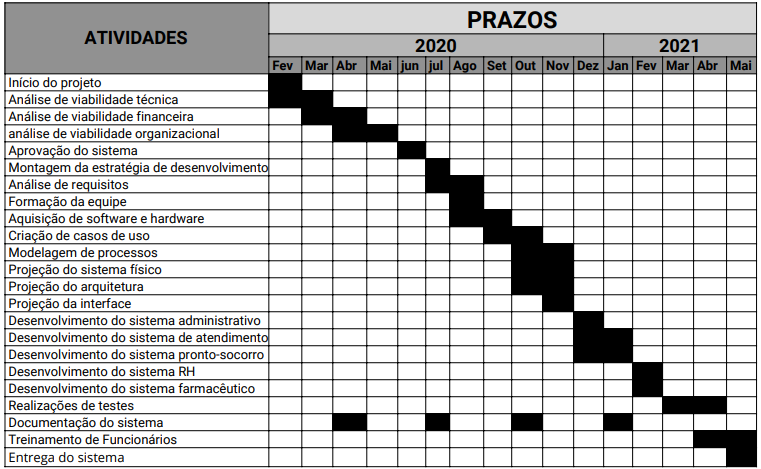
\includegraphics[width=15cm]{Cronograma.png} \\
               
              \end{center}
             \end{figure}
          
       \subsection{Or\c{c}amento }
% Please add the following required packages to your document preamble:
% \usepackage[normalem]{ulem}
% \useunder{\uline}{\ul}{}
\begin{table}[H]
       \centering
       \caption{Orçamento para construção do sistema}
       \begin{tabular}{|l|l|l|l|}
       \hline
       {\ul \textbf{Quantidade}} & {\ul \textbf{Componentes}}         & {\ul \textbf{Preço/unidade (R\$)}} & {\ul \textbf{Valor total (R\$)}} \\ \hline
                                 & \textbf{Hardware}                  &                                    &                                  \\ \hline
       110                       & Monitores                          & 300,00                             & 33.000,00                        \\ \hline
       110                       & Microcomputadores                  & 2.200,00                           & 242.000,00                       \\ \hline
       70                        & Impressoras                        & 300,00                             & 21.000,00                        \\ \hline
       18                        & Impressoras multifuncional         & 900,00                             & 16.200,00                        \\ \hline
       1                         & Smart TV de 40 polegadas           & 1.200,00                           & 1.200,00                         \\ \hline
       8                         & GPS                                & 300,00                             & 2.400,00                         \\ \hline
       6                         & Roteador Wireless                  & 150,00                             & 1.200,00                         \\ \hline
       1                         & Sevidor                            & 15.000,00                          & 15.000,00                        \\ \hline
       7                         & Switch                             & 150                                & 1.050,00                         \\ \hline
                                 & \textbf{}                          &                                    & \textbf{332.000,00}              \\ \hline
                                 & \textbf{Software}                  &                                    &                                  \\ \hline
       110                       & Sistemas operacionais proprietário & 600,00                             & 66.000,00                        \\ \hline
       50                        & Pacotes Office                     & 300,00                             & 15.000,00                        \\ \hline
       1                         & Hospedagem de site                 & 12.000,00                          & 12.000,00                        \\ \hline
       1                         & Domínio do site                    & 150,00                             & 150,00                           \\ \hline
                                 & \textbf{}                          &                                    & \textbf{93.150,000}              \\ \hline
                                 & \textbf{Pessoas}                   &                                    &                                  \\ \hline
       15                        & Programadores                      & 30.000,00                          & 450.000,00                       \\ \hline
       3                         & Analista de sistema                & 200.000,00                         & 600.000,00                       \\ \hline
       1                         & Chefe do Projeto                   & 300.000,00                         & 300.000,00                       \\ \hline
       4                         & Arquitetos de software             & 120.000,00                         & 480.000,00                       \\ \hline
       2                         & Projetista                         & 30.000,00                          & 60.000,00                        \\ \hline
       2                         & Avaliadores de Qualidade           & 15.000,00                          & 30.000,00                        \\ \hline
       5                         & Funcionários de manutenção         & 25.000,00                          & 125.000,00                       \\ \hline
                                 & \textbf{}                          &                                    & \textbf{2.045.000,00}            \\ \hline
                                 &                                    & \textbf{Total}                     & \textbf{2.470.150,00}            \\ \hline
       \end{tabular}
       \end{table}

       \subsection{Recomenda\c{c}\~{o}es}
       É importante que seja seguido o cronograma, que seja adquirido todos os equipamentos necessários, e também a contratação de todos os funcionários exigidos na tabela 2.2 de orçamento. Essas recomendações são extremamente necessária para o funcionamento de forma correta do sistema.
       \subsection{Conclus\~{a}o de Viabilidade}
       Considerando que o cronograma das tarefas do sistema a ser desenvolvido atende às necessidades, e os custos de construção se encaixa dentro do orçamento do hospital. Sendo assim o projeto é viável do ponto de vista técnico, econômico e organizacional.